% TJMJ Technical Manual — English Edition
% Compile: xelatex × 3
\documentclass[11pt,a4paper]{article}
\usepackage[UTF8]{ctex}
\setCJKmainfont{SimSun}[BoldFont=SimHei,ItalicFont=KaiTi]
\setCJKmonofont{FangSong}
\usepackage{fontspec}\setmainfont{Times New Roman}
\renewcommand{\ttdefault}{lmtt}

\usepackage{geometry}
\geometry{top=2.2cm,bottom=2.2cm,left=2.5cm,right=2.5cm}
\usepackage{fancyhdr}\pagestyle{fancy}\fancyhf{}
\fancyhead[L]{\small TJMJ Technical Manual (English)}
\fancyhead[R]{\small\thepage}
\renewcommand{\headrulewidth}{0.4pt}
\setlength{\parskip}{2pt}
\renewcommand{\baselinestretch}{1.0}
\usepackage[compact]{titlesec}
\titlespacing{\section}{0pt}{6pt}{3pt}
\titlespacing{\subsection}{0pt}{3pt}{1pt}
\titlespacing{\subsubsection}{0pt}{3pt}{1pt}

\usepackage{amsmath,amssymb,mathtools}
\usepackage{graphicx}
\usepackage[table]{xcolor}
\usepackage{booktabs,array,multirow,tabularx,longtable}
\usepackage{enumitem}
\setlist{nosep,leftmargin=*}
\usepackage{hyperref}
\hypersetup{colorlinks=true,linkcolor=black,urlcolor=blue,citecolor=blue}
\usepackage{float}
\usepackage{multicol}
\usepackage{caption,subcaption}
\usepackage{listings}
\lstset{basicstyle=\ttfamily\footnotesize,breaklines=true,frame=single,rulecolor=\color{gray!40},backgroundcolor=\color{gray!5},keywordstyle=\color{blue}\bfseries,commentstyle=\color{green!50!black},stringstyle=\color{red!70!black},showstringspaces=false,numbers=left,numberstyle=\tiny\color{gray},numbersep=5pt,tabsize=2,language={}}
\usepackage{tikz}
\usetikzlibrary{shapes,arrows,positioning,fit,calc,backgrounds}
\tikzset{
  b/.style={rectangle,draw,rounded corners=1pt,fill=blue!5,text width=2.8cm,minimum height=0.9cm,align=center,font=\footnotesize},
  sb/.style={rectangle,draw,rounded corners=1pt,fill=green!5,text width=2cm,minimum height=0.7cm,align=center,font=\scriptsize},
  arr/.style={->,>=stealth,thick},
  cld/.style={ellipse,draw,fill=gray!10,minimum width=3cm,minimum height=1.2cm,align=center,font=\footnotesize},
  cli/.style={rectangle,draw,fill=blue!5,text width=2.5cm,minimum height=0.8cm,align=center,font=\footnotesize},
  srv/.style={rectangle,draw,fill=orange!10,text width=2.5cm,minimum height=0.8cm,align=center,font=\footnotesize},
}
\usepackage{sectsty}
\allsectionsfont{\color{blue!70!black}}

\title{\bfseries\LARGE\color{blue!60!black} Taojiang Classic Wang Mahjong (TJMJ)\\[4pt]
       \large\color{blue!50!black} Full-Stack Real-Time Web Platform — Technical Report}
\author{%
  \begin{tabular}{c}
  \small\textbf{Jintian Xia}$^{1}$ \quad \textbf{Siyuan Liu}$^{1}$ \quad \textbf{Jianghong Xiang}$^{1}$ \quad \textbf{Zhuangwei Zeng}$^{1}$ \\
  \small\textbf{Jian Hu}$^{1}$ \quad \textbf{Yangyang Song}$^{1}$ \quad \textbf{Hao Wen}$^{1}$ \quad \textbf{Xiaobing Yang}$^{1}$ \quad \textbf{Erma Li}$^{1}$ \\[4pt]
  \small\textbf{Jaijai C}$^{1,\dagger}$ \\[2pt]
  \small$^{1}$\textit{School of Entertainment Computing, TJMJ Lab, Taojiang, Hunan, China} \\
  \small$\dagger$\textit{Corresponding author: }\texttt{jaijai.c@tjmj.dev} \\[2pt]
  \small\texttt{\color{blue}https://github.com/JaijaiC/TJMJ}
  \end{tabular}
}
\date{}

\begin{document}
\maketitle

\begin{tikzpicture}[overlay,remember picture]
  \foreach \y in {0,0.8,1.6,2.4} {
    \node[font=\tiny,text=gray!30] at ([shift={(0.8cm,-\y cm)}]current page.north east) {$\diamond$};
    \node[font=\tiny,text=gray!30] at ([shift={(-0.8cm,-\y cm)}]current page.north west) {$\diamond$};
  }
\end{tikzpicture}

\vspace{-8pt}
\begin{center}
{\color{cyan!60!black}\rule{\linewidth}{1.5pt}}\\[2pt]
\begin{minipage}{0.95\linewidth}
{\centering\small\textbf{\color{orange!80!black}Abstract}\par}
\vspace{4pt}
\color{black!80}\setlength{\parindent}{2em}
Taojiang Mahjong, as the most representative local chess-and-card cultural symbol of the Taojiang region in Hunan Province, embodies centuries of leisure wisdom and social memory of the local people. Its unique "Da Shai Ban Wang" wildcard mechanism, "Zha Niao" multiplier scoring, and "Menzi" cumulative pattern system preserve remarkable strategic depth and gaming enjoyment while simplifying the tile set to 108 pieces (excluding wind and flower tiles). However, this precious intangible cultural heritage has long lacked a dedicated digital carrier — existing mahjong platforms either misalign with local rules, are heavily commercialized, or remain technologically closed, making it difficult for Taojiang natives away from home to find a familiar game and threatening the continuity of local cultural transmission. The TJMJ project was born precisely to fill this gap, injecting new vitality into Taojiang Mahjong through modern web technology.

The platform's frontend adopts a Vue 3 Composition API single-page architecture with Vite 8 build toolchain, while the backend leverages a Node.js WebSocket server for server-authoritative multiplayer real-time battles. Voice communication employs WebRTC P2P mesh topology supplemented by Agora SD-RTN relay. The system fully implements the Taojiang local mahjong rule system, supporting single-player AI, four-player online, and spectator modes. Core algorithms include an $\mathcal{O}(3^k)$ recursive backtracking winning-hand detection engine (sub-millisecond measured runtime), heuristic NPC discard strategy, and a differential client-server hand-tile synchronization algorithm. This paper provides complete system architecture diagrams, protocol definitions, mathematical formulas, algorithm pseudocode, cross-platform compatibility solutions, and performance benchmarks.

The project is fully open-source (approximately 4,200 lines of code), with the frontend deployed on GitHub Pages and the backend tunneled via ngrok — no installation required, click-and-play. TJMJ represents not only a formal modeling and technical implementation of Taojiang Mahjong rules, but also an active exploration of revitalizing local traditional culture through internet technology. We hope this platform can contribute modestly to the digital dissemination of Taojiang's cultural heritage, allowing Taojiang natives wherever they may be to feel the warmth of home in a game of mahjong, and enabling more friends from afar to discover and fall in love with this uniquely charming local chess-and-card art.
\end{minipage}\\[2pt]
{\color{cyan!60!black}\rule{\linewidth}{0.5pt}}\\[2pt]
\begin{minipage}{0.95\linewidth}
\small\textbf{\color{blue!60!black}Keywords:} \textbf{Mahjong $\cdot$ Full-Stack Web $\cdot$ Real-Time Multiplayer $\cdot$ WebRTC $\cdot$ Node.js $\cdot$ Vue 3 $\cdot$ Recursive Backtracking $\cdot$ Cross-Platform} \\
\textbf{\color{blue!60!black}Test Status:} $\blacksquare$ Verified \quad $\square$ Pending \quad $\triangle$ Partial \\[2pt]
\textbf{\color{blue!60!black}Repository:} \url{https://github.com/JaijaiC/TJMJ} \\
\textbf{\color{blue!60!black}Live Demo:} \url{https://jaijaic.github.io/TJMJ/} \\
\textbf{\color{blue!60!black}GitHub:} \url{https://github.com/JaijaiC/TJMJ}
\end{minipage}\\[4pt]
{\color{cyan!60!black}\rule{\linewidth}{0.5pt}}
\end{center}

\vspace{6pt}
\begin{center}
{\small\color{gray}\today}
\end{center}

\newpage
\renewcommand{\contentsname}{\begin{center}Contents\end{center}}
\tableofcontents
\newpage

% ===================================================================
\section{Introduction}
% ===================================================================

\subsection{Background and Motivation}

Chinese Mahjong is one of the most widely played tabletop game genres in the world, with rules evolving into dozens of regional variants over centuries of geographic diffusion. The "Classic Wang Mahjong" of Taojiang, Hunan, is a uniquely distinctive branch: it uses a simplified 108-tile set (Characters/Bamboos/Dots only, excluding Wind and Flower tiles), dynamically determines a wildcard (Joker) through the "Ban Wang" mechanism, applies the "Zha Niao" post-win multiplier scoring, and allows multiple "Menzi" (bonus patterns) to accumulate. These rules collectively shape Taojiang Mahjong's fast-paced, intense, and unpredictable gameplay rhythm, deeply beloved by local communities.

However, the digital ecosystem for Taojiang Mahjong has long been vacant. Only a handful of commercial apps such as Xianyi offer Yiyang-region mahjong, with significant deficiencies:
\[
\left\{\begin{minipage}{0.88\linewidth}
\begin{enumerate}[nosep,leftmargin=*]
  \item Mandatory registration and login with lengthy onboarding flows;
  \item Cluttered interface design with heavy advertising interruptions;
  \item Incomplete alignment of rule implementations with authentic Taojiang local play (e.g., missing Zha Niao and Ban Wang core mechanics);
  \item Lack of modern interaction features such as drag-to-reorder hand tiles, real-time voice, and text danmaku;
  \item Closed-source, unavailable for secondary development or academic research.
\end{enumerate}
\end{minipage}
\right.
\]
Furthermore, the WeChat Mini Program path is blocked because chess-and-card games require regulatory filing currently unavailable to individuals, and game engines like Cocos have high entry barriers with low development efficiency.

TJMJ emerged in response — a fully open-source, install-free, click-and-play web mahjong platform. Built upon a Vue 3 Composition API + Vite 8 frontend and Node.js WebSocket backend, it fully implements all Taojiang Mahjong rules and provides three game modes: single-player (vs AI), four-player real-time online battles, and spectating. This paper serves as the complete technical documentation of the platform, covering system architecture, game rules, algorithm implementation, multiplayer infrastructure, cross-platform compatibility, and performance evaluation.

\textbf{Key Contributions}:
\begin{enumerate}[nosep]
  \item Complete mathematical formalization of Taojiang Mahjong rules — including tile-set encoding, dice mechanics, wildcard computation, action priority, scoring model, and Zha Niao formula;
  \item Production-grade full-stack architecture — server-authoritative multiplayer game system achieving sub-100ms state synchronization latency via JSON over WebSocket;
  \item Recursive backtracking winning-hand detection engine — $\mathcal{O}(3^k)$ worst-case complexity, measured $<$1\,ms, with ting detection and NPC heuristic decision-making;
  \item Fault-tolerant multiplayer infrastructure — exponential backoff reconnection, server-side 10-second action timeout deadlock prevention, URL-parameter room state persistence;
  \item Comprehensive cross-platform adaptation — solving practical issues including iOS Safari click events, AudioContext suspension, Android dynamic address bar, and CSS transform breaking fixed positioning.
\end{enumerate}

\subsection{Project Scale}

Table~\ref{tab:scale} lists the size statistics of core source code files.

\begin{table}[H]
\centering
\caption{Core Code Scale}
\label{tab:scale}
\small
\begin{tabular}{@{}lrr@{}}
\toprule
\textbf{File} & \textbf{Lines} & \textbf{Responsibility} \\
\midrule
\texttt{frontend/src/App.vue} & 2602 & Main UI + Game Logic + CSS \\
\texttt{server/GameRoom.js} & 494 & Multiplayer Room State Machine \\
\texttt{server/index.js} & 247 & WebSocket Server Entry \\
\texttt{frontend/src/ai/NpcStrategy.js} & 227 & NPC Discard Decision AI \\
\texttt{frontend/src/network/client.js} & 224 & Network Layer (reconnect/heartbeat/throttle) \\
\texttt{frontend/src/core/HuCalculator.js} & 208 & Winning-Hand Detection Engine \\
\texttt{frontend/src/core/RuleChecker.js} & 142 & Chi/Peng/Gang Rule Checker \\
\texttt{frontend/src/utils/speech.js} & 100 & Voice Announcement System \\
\midrule
\textbf{Total} & \textbf{4244} & — \\
\bottomrule
\end{tabular}
\end{table}

\newpage
% ===================================================================
\section{Related Work Comparison}
% ===================================================================

Table~\ref{tab:platforms} compares core feature differences among existing digital mahjong platforms. TJMJ demonstrates significant advantages across four dimensions: Taojiang rule fidelity, registration-free experience, open-source accessibility, and interaction innovation (drag-to-reorder tiles, real-time voice, text danmaku).

\begin{table}[H]
\centering
\caption{Digital Mahjong Platform Feature Comparison}
\label{tab:platforms}
\footnotesize
\begin{tabular}{@{}lccccc@{}}
\toprule
\textbf{Feature} & \textbf{Xianyi} & \textbf{MajSoul} & \textbf{Wuhan MJ} & \textbf{Open-MJ} & \textbf{TJMJ} \\
\midrule
Taojiang Rules & Partial & $\times$ & $\times$ & $\times$ & \checkmark \\
No Registration & $\times$ & $\times$ & \checkmark & \checkmark & \checkmark \\
Open Source & $\times$ & $\times$ & $\times$ & \checkmark & \checkmark \\
Drag-to-Reorder Tiles & $\times$ & $\times$ & $\times$ & $\times$ & \checkmark \\
Real-Time Voice & $\times$ & $\times$ & $\times$ & $\times$ & \checkmark \\
Text Danmaku & $\times$ & $\times$ & $\times$ & $\times$ & \checkmark \\
Spectator Mode & $\times$ & \checkmark & $\times$ & $\times$ & \checkmark \\
AI Opponents & $\times$ & \checkmark & $\times$ & $\times$ & \checkmark \\
Web-Native & $\times$ & \checkmark & \checkmark & \checkmark & \checkmark \\
\bottomrule
\end{tabular}
\end{table}

\subsection{Web Real-Time Gaming Technology Stack}

TJMJ's choices are grounded in the following technology maturity considerations: WebSocket (RFC~6455) provides full-duplex low-overhead communication, reducing latency by approximately 80\% compared to HTTP long-polling; the WebRTC standard offers browser-native P2P audio/video capabilities with STUN/TURN infrastructure for cross-NAT traversal; Vue 3 Composition API's reactive state management naturally suits incremental updates in complex UIs; Vite 8's native ESM dev server and Rolldown bundler deliver ultra-fast cold starts and build experiences.

\newpage
% ===================================================================
\section{System Architecture}
% ===================================================================

\subsection{Overall Architecture}

TJMJ adopts a classic three-tier B/S architecture, organized top-down into the presentation layer, network layer, and application service layer. Figure~\ref{fig:arch} illustrates the complete data pathway from browser to server.

The \textbf{Presentation Layer} runs in the player's browser, rendering the game interface, handling user interactions (clicks, drags, voice input), and communicating with the application server via WebSocket. The \textbf{Network Layer} bears three critical channels: GitHub Pages provides HTTPS distribution of static assets, the ngrok TCP tunnel penetrates public-network WebSocket traffic to the local server, and WebRTC P2P direct connections carry real-time voice streams. The \textbf{Application Server} serves as the system's core hub — a single Node.js process handles all WebSocket message routing and game room management, while dynamically generating Agora tokens via HMAC-SHA1 to facilitate NAT traversal. The \textbf{Game Engine} employs a dual-end deployment strategy — the same rule-checking code (HuCalculator, RuleChecker, mjLogic) runs both on the frontend to provide instant feedback and on the server in authoritative mode to prevent cheating.

\begin{figure}[H]
\centering
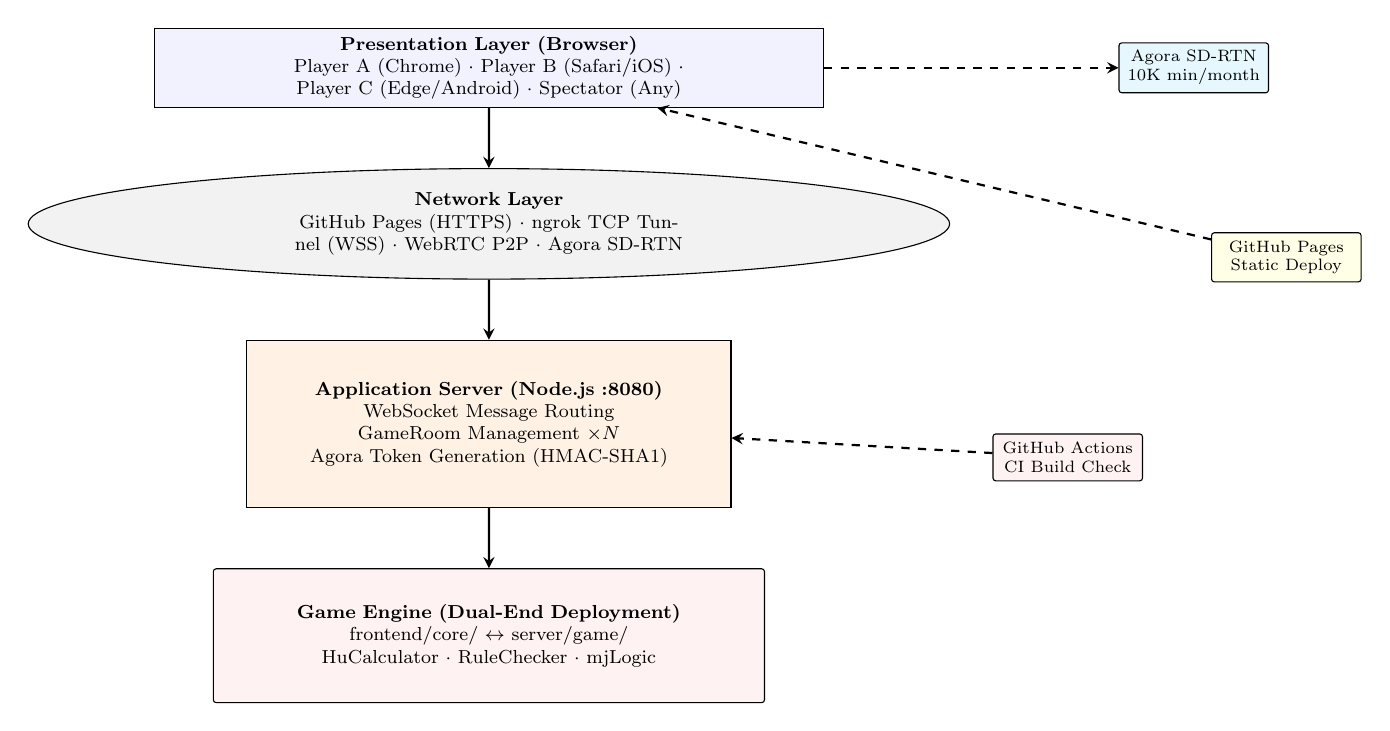
\begin{tikzpicture}[node distance=0.9cm, scale=0.85, every node/.style={transform shape}]
  \node[cli,minimum width=10cm,text width=9.5cm] (c) {\textbf{Presentation Layer (Browser)}\\Player A (Chrome) $\cdot$ Player B (Safari/iOS) $\cdot$ Player C (Edge/Android) $\cdot$ Spectator (Any)};
  \node[cld,below=of c,minimum width=10cm,text width=9.5cm] (n) {\textbf{Network Layer}\\GitHub Pages (HTTPS) $\cdot$ ngrok TCP Tunnel (WSS) $\cdot$ WebRTC P2P $\cdot$ Agora SD-RTN};
  \node[srv,below=of n,text width=7cm,minimum height=2.5cm] (s) {\textbf{Application Server (Node.js :8080)}\\WebSocket Message Routing\\GameRoom Management $\times N$\\Agora Token Generation (HMAC-SHA1)};
  \node[b,below=of s,text width=8cm,minimum height=2cm,fill=red!5] (g) {\textbf{Game Engine (Dual-End Deployment)}\\frontend/core/ $\leftrightarrow$ server/game/\\HuCalculator $\cdot$ RuleChecker $\cdot$ mjLogic};
  \draw[arr] (c) -- (n);
  \draw[arr] (n) -- (s);
  \draw[arr] (s) -- (g);
  \node[sb,right=of n,xshift=3cm,yshift=-0.5cm,fill=yellow!10] (gh) {GitHub Pages\\Static Deploy};
  \node[sb,right=of s,xshift=3cm,yshift=-0.5cm,fill=red!5] (ci) {GitHub Actions\\CI Build Check};
  \node[sb,right=of c,xshift=3.5cm,fill=cyan!10] (v) {Agora SD-RTN\\10K min/month};
  \draw[arr,dashed] (gh) -- (c);
  \draw[arr,dashed] (ci) -- (s);
  \draw[arr,dashed] (c.east) -- (v.west);
\end{tikzpicture}
\caption{System Architecture Overview}
\label{fig:arch}
\end{figure}

\subsection{Frontend Component Architecture}

The Vue 3 frontend centers on a single master component \texttt{App.vue} (2,602 lines), consolidating all UI templates, game logic, and CSS styles into one single-file component — yielding extremely high development efficiency during rapid iteration. Figure~\ref{fig:fe} depicts the component dependency graph. The core game engine (core/) handles winning-hand detection and rule checking; the network layer (network/) manages WebSocket communication and reconnection; the AI module (ai/) drives NPC decisions; the utilities module (utils/) provides shuffle logic and voice announcements; static assets (public/) contain tile graphics, sound effects, and documentation.

\begin{figure}[H]
\centering
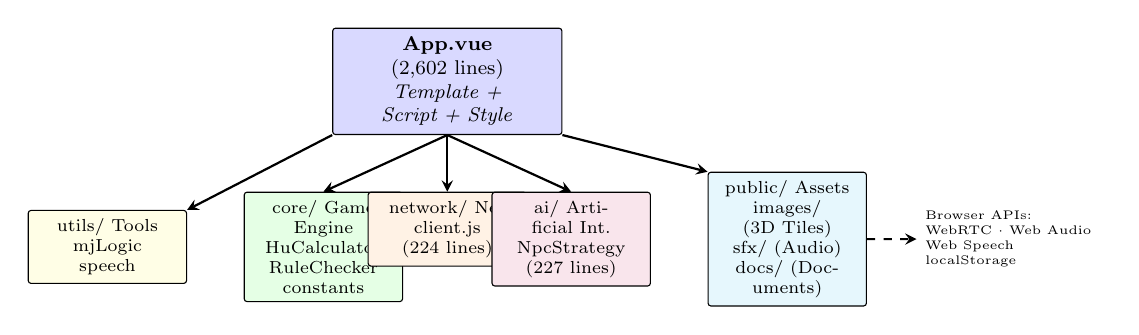
\begin{tikzpicture}[node distance=0.7cm, scale=0.9, every node/.style={transform shape}]
  \node[b,fill=blue!15,text width=3cm,minimum height=1.5cm] (app) {\textbf{App.vue}\\(2,602 lines)\\\textit{Template + Script + Style}};
  \node[sb,below left=0.8cm and -1cm of app,fill=green!10] (core) {core/ Game Engine\\HuCalculator\\RuleChecker\\constants};
  \node[sb,below=0.8cm of app,fill=orange!10] (net) {network/ Net\\client.js\\(224 lines)};
  \node[sb,below right=0.8cm and -1cm of app,fill=purple!10] (ai) {ai/ Artificial Int.\\NpcStrategy\\(227 lines)};
  \node[sb,left=0.8cm of core,fill=yellow!10] (ut) {utils/ Tools\\mjLogic\\speech};
  \node[sb,right=0.8cm of ai,fill=cyan!10] (as) {public/ Assets\\images/ (3D Tiles)\\sfx/ (Audio)\\docs/ (Documents)};
  \draw[arr] (app.south) -- (core.north); \draw[arr] (app.south) -- (net.north); \draw[arr] (app.south) -- (ai.north);
  \draw[arr] (app.south west) -- (ut.north east); \draw[arr] (app.south east) -- (as.north west);
  \node[right=of as,font=\tiny,text width=2.5cm] (api) {Browser APIs:\\WebRTC $\cdot$ Web Audio\\Web Speech\\localStorage};
  \draw[arr,dashed] (as.east) -- (api.west);
\end{tikzpicture}
\caption{Frontend Component Dependency Graph}
\label{fig:fe}
\end{figure}

\subsection{Backend Service Architecture}

The server consists of two core files: \texttt{index.js} (247 lines) implements WebSocket message routing and Agora token generation, while \texttt{GameRoom.js} (494 lines) implements the room finite state machine. Figure~\ref{fig:be} illustrates the message processing pipeline: client messages enter the WebSocket server, pass through the message router, and are dispatched to corresponding handlers based on the type field. Each active room maintains an independent GameRoom instance managing the players array, hands state, exposed melds, and pendingActions interception queue.

\begin{figure}[H]
\centering
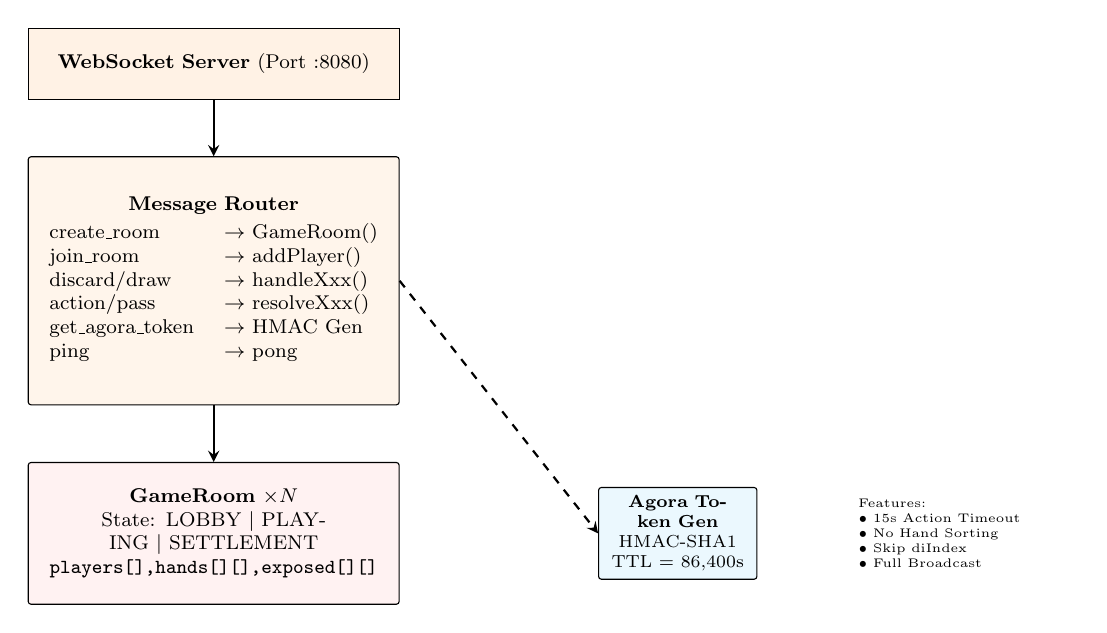
\begin{tikzpicture}[node distance=0.8cm, scale=0.9, every node/.style={transform shape}]
  \node[srv,text width=5cm,minimum height=1cm] (wss) {\textbf{WebSocket Server} (Port :8080)};
  \node[b,below=of wss,text width=5cm,minimum height=3.5cm,fill=orange!8] (r) {\textbf{Message Router}\\[2pt]\begin{tabular}{@{}ll@{}}
    create\_room & $\to$ GameRoom() \\
    join\_room   & $\to$ addPlayer() \\
    discard/draw & $\to$ handleXxx() \\
    action/pass  & $\to$ resolveXxx() \\
    get\_agora\_token & $\to$ HMAC Gen \\
    ping         & $\to$ pong \\
  \end{tabular}};
  \node[b,below=of r,text width=5cm,minimum height=2cm,fill=red!5] (rm) {\textbf{GameRoom $\times N$}\\State: LOBBY $|$ PLAYING $|$ SETTLEMENT\\\texttt{players[],hands[][],exposed[][]}};
  \node[sb,right=of rm,xshift=2cm,fill=cyan!8] (t) {\textbf{Agora Token Gen}\\HMAC-SHA1\\TTL = 86,400s};
  \draw[arr] (wss) -- (r); \draw[arr] (r) -- (rm); \draw[arr,dashed] (r.east) -- (t.west);
  \node[right=of t,xshift=0.5cm,font=\tiny,text width=3cm] {Features:\\$\bullet$ 15s Action Timeout\\$\bullet$ No Hand Sorting\\$\bullet$ Skip diIndex\\$\bullet$ Full Broadcast};
\end{tikzpicture}
\caption{Backend Service Architecture}
\label{fig:be}
\end{figure}

\subsection{Communication Protocol Stack}

Figure~\ref{fig:stack} depicts the complete communication stack from application to transport layer.

\begin{figure}[H]
\centering
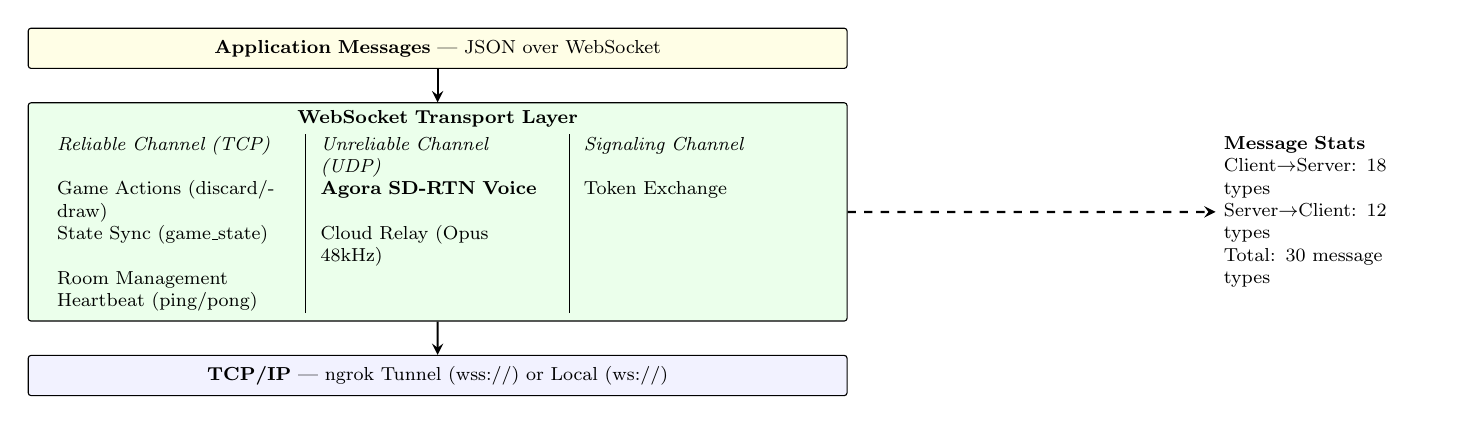
\begin{tikzpicture}[node distance=0.5cm, scale=0.85, every node/.style={transform shape}]
  \node[b,fill=yellow!10,text width=12cm,minimum height=0.6cm] (a) {\textbf{Application Messages} — JSON over WebSocket};
  \node[b,fill=green!8,text width=12cm,minimum height=2.5cm,below=of a] (ws) {\textbf{WebSocket Transport Layer}\\[2pt]\begin{tabular}{@{}p{3.5cm}|p{3.5cm}|p{3.5cm}@{}}
    \textit{Reliable Channel (TCP)} & \textit{Unreliable Channel (UDP)} & \textit{Signaling Channel} \\
    Game Actions (discard/draw) & \textbf{Agora SD-RTN Voice} & Token Exchange \\
    State Sync (game\_state) & Cloud Relay (Opus 48kHz) & \\
    Room Management & & \\
    Heartbeat (ping/pong) & &
  \end{tabular}};
  \node[b,fill=blue!5,text width=12cm,minimum height=0.6cm,below=of ws] (t) {\textbf{TCP/IP} — ngrok Tunnel (wss://) or Local (ws://)};
  \draw[arr] (a) -- (ws); \draw[arr] (ws) -- (t);
  \node[font=\footnotesize,right=of ws,xshift=5cm,text width=3cm] (n) {\textbf{Message Stats}\\Client$\to$Server: 18 types\\Server$\to$Client: 12 types\\Total: 30 message types};
  \draw[arr,dashed] (ws.east) -- (n.west);
\end{tikzpicture}
\caption{Communication Protocol Stack}
\label{fig:stack}
\end{figure}

\subsection{WebSocket Message Protocol}

Table~\ref{tab:proto} lists the complete definitions of all 30 message types.

\begin{table}[H]
\centering
\caption{Complete WebSocket Message Protocol}
\label{tab:proto}
\footnotesize
\begin{tabular}{@{}llp{5cm}@{}}
\toprule
\textbf{Message Type} & \textbf{Direction} & \textbf{Description} \\
\midrule
\texttt{create\_room}    & C$\to$S & Create room (optional 4-digit code) \\
\texttt{join\_room}      & C$\to$S & Join room (8888 = test room) \\
\texttt{ready}           & C$\to$S & Ready (auto-start when 4 ready) \\
\texttt{ready\_next}     & C$\to$S & Confirm continue (all 4 → new round) \\
\texttt{discard}         & C$\to$S & Discard tile (with tile value) \\
\texttt{draw}            & C$\to$S & Draw request \\
\texttt{action}          & C$\to$S & Chi/Peng/Gang/Hu (with action + combo) \\
\texttt{pass}            & C$\to$S & Pass interception \\
\texttt{chat}            & C$\leftrightarrow$S & Text danmaku (with text + fromName) \\
\texttt{emoji}           & C$\leftrightarrow$S & Emoji (with icon + target) \\
\texttt{get\_agora\_token}& C$\to$S & Request Agora voice token \\
\texttt{update\_avatar}  & C$\to$S & Avatar sync \\
\texttt{join\_spectate}  & C$\to$S & Join as spectator \\
\texttt{ping}            & C$\to$S & Heartbeat \\
\texttt{pay}             & C$\to$S & Manual score transfer \\
\midrule
\texttt{room\_created}   & S$\to$C & Room created (returns roomId) \\
\texttt{room\_joined}    & S$\to$C & Room joined \\
\texttt{room\_players}   & S$\to$C & Player list update \\
\texttt{game\_start}     & S$\to$C & Game start (hand + wangTile + dice) \\
\texttt{game\_state}     & S$\to$C & Real-time state sync \\
\texttt{action\_prompt}  & S$\to$C & Request player action \\
\texttt{drew\_tile}      & S$\to$C & Tile drawn \\
\texttt{round\_end}      & S$\to$C & Round end (all hands revealed) \\
\texttt{pong}            & S$\to$C & Heartbeat reply \\
\texttt{agora\_token}    & S$\to$C & Agora voice token \\
\texttt{avatar\_updated} & S$\to$C & Avatar synced \\
\texttt{game\_end}       & S$\to$C & 16-round finale \\
\bottomrule
\end{tabular}
\end{table}

\subsection{Voice Architecture}

Multiplayer voice uses Agora SD-RTN (Software-Defined Real-Time Network) cloud relay. Each player joins the same Agora channel (named \texttt{tjmj\_\{roomId\}}). Audio streams are captured locally via \texttt{createMicrophoneAudioTrack}, published to the Agora cloud, and automatically distributed to all other channel members. Tokens are generated server-side using HMAC-SHA1 with 24-hour validity. This architecture eliminates all P2P connection management complexity and NAT traversal issues.

\begin{figure}[H]
\centering
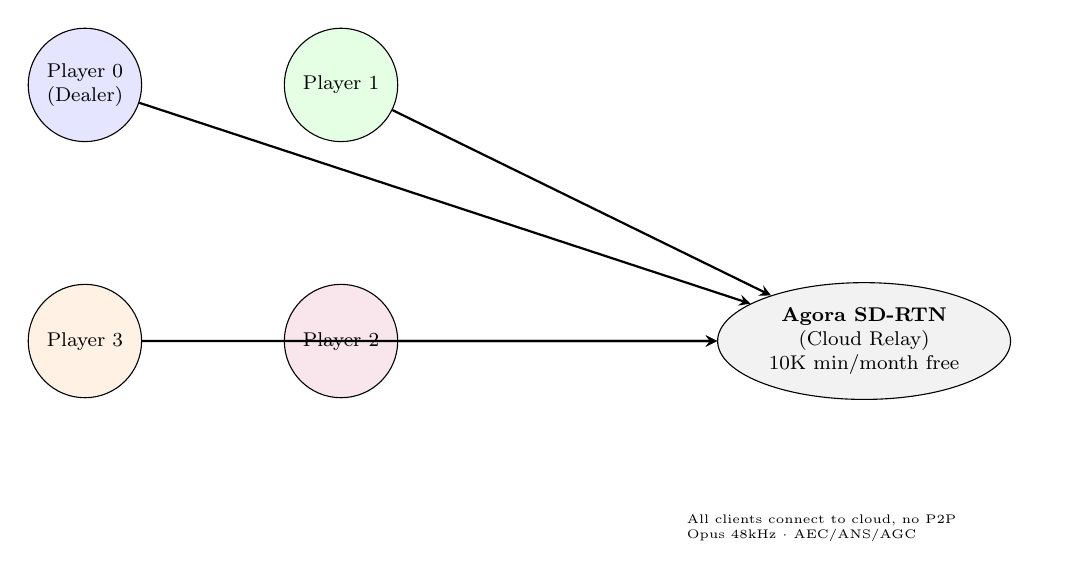
\begin{tikzpicture}[node distance=2cm, scale=0.9, every node/.style={transform shape}]
  \node[circle,draw,fill=blue!10,minimum size=1.6cm,font=\footnotesize,align=center] (p0) {Player 0\\(Dealer)};
  \node[circle,draw,fill=green!10,minimum size=1.6cm,font=\footnotesize,align=center,right=of p0] (p1) {Player 1};
  \node[circle,draw,fill=orange!10,minimum size=1.6cm,font=\footnotesize,align=center,below=of p0] (p3) {Player 3};
  \node[circle,draw,fill=purple!10,minimum size=1.6cm,font=\footnotesize,align=center,below=of p1] (p2) {Player 2};
  \node[cld,right=of p2,xshift=2.5cm,minimum width=4cm] (cloud) {\textbf{Agora SD-RTN}\\(Cloud Relay)\\10K min/month free};
  \draw[arr] (p0) -- (cloud); \draw[arr] (p1) -- (cloud);
  \draw[arr] (p2) -- (cloud); \draw[arr] (p3) -- (cloud);
  \node[font=\tiny,below=of cloud,yshift=0.5cm,text width=5cm] {All clients connect to cloud, no P2P\\Opus 48kHz $\cdot$ AEC/ANS/AGC};
\end{tikzpicture}
\caption{Agora Cloud Voice Architecture}
\label{fig:voice}
\end{figure}

\subsection{Deployment Architecture}

Figure~\ref{fig:deploy} illustrates the complete deployment flow from development to production.

\begin{figure}[H]
\centering
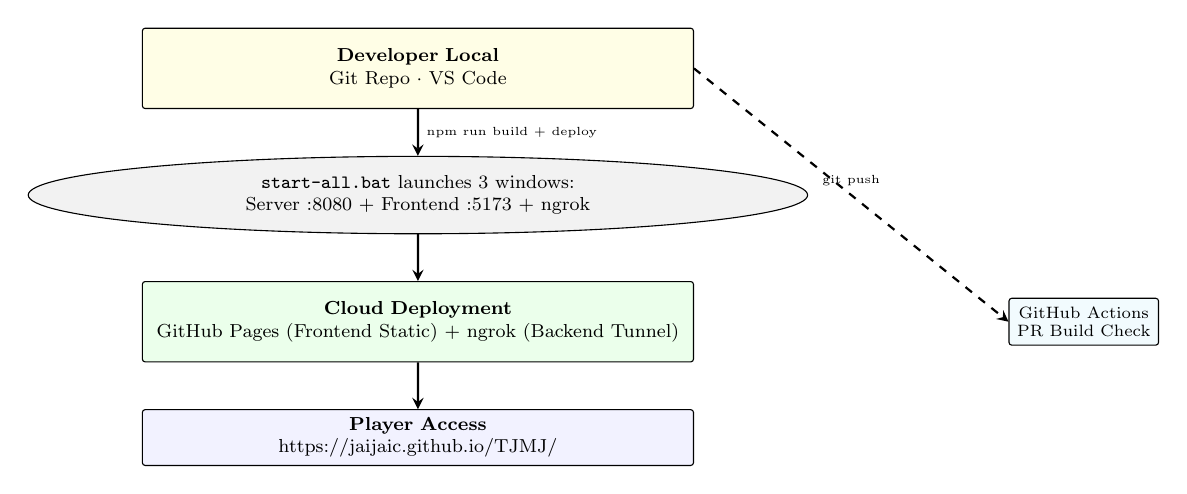
\begin{tikzpicture}[node distance=0.7cm, scale=0.85, every node/.style={transform shape}]
  \node[b,fill=yellow!10,text width=8cm,minimum height=1.2cm] (dev) {\textbf{Developer Local}\\Git Repo $\cdot$ VS Code};
  \node[cld,below=of dev,text width=8cm,minimum height=0.8cm] (cmd) {\texttt{start-all.bat} launches 3 windows: Server :8080 + Frontend :5173 + ngrok};
  \node[b,fill=green!8,text width=8cm,minimum height=1.2cm,below=of cmd] (deploy) {\textbf{Cloud Deployment}\\GitHub Pages (Frontend Static) + ngrok (Backend Tunnel)};
  \node[b,fill=blue!5,text width=8cm,minimum height=0.8cm,below=of deploy] (user) {\textbf{Player Access}\\https://jaijaic.github.io/TJMJ/};
  \draw[arr] (dev) -- (cmd) node[midway,right,font=\tiny] {npm run build + deploy};
  \draw[arr] (cmd) -- (deploy);
  \draw[arr] (deploy) -- (user);
  \node[sb,right=of deploy,xshift=4cm,fill=cyan!5] (act) {GitHub Actions\\PR Build Check};
  \draw[arr,dashed] (dev.east) -- (act.west) node[midway,above,font=\tiny] {git push};
\end{tikzpicture}
\caption{Deployment Architecture}
\label{fig:deploy}
\end{figure}

\newpage
% ===================================================================
\section{Game Rules and Mathematical Model}
% ===================================================================

\subsection{Tile Set Definition and Encoding}

Define the tile set $\mathcal{T} = \{11,12,\ldots,19,21,\ldots,29,31,\ldots,39\}$. The encoding rule is $t = 10s + v$, where $s \in \{1,2,3\}$ denotes the suit category (1=Characters, 2=Bamboos, 3=Dots) and $v \in \{1,\ldots,9\}$ denotes the face value. Each tile has 4 identical copies, totaling $|\mathcal{T}|=108$.

Define the "Jiang" (pair) tile set as $\mathcal{J} = \{t \in \mathcal{T} \mid t \bmod 10 \in \{2,5,8\}\}$. With 3 suits, 3 face values per suit, and 4 copies each, $|\mathcal{J}| = 3 \times 3 \times 4 = 36$. A Jiang pair is a necessary element of a winning hand.

\subsection{Dice Mechanics and Dealing}

At the start of a round, two fair six-sided dice are rolled, with values denoted $d_1, d_2$ ($d_1 \leq d_2$). The sum $S = d_1 + d_2$ determines the starting wall. Counting counterclockwise from the dealer $P_0$, the wall before the player corresponding to $S$ becomes the starting wall ($P_0$ for 1,5,9; $P_1$ for 2,6,10; $P_2$ for 3,7,11; $P_3$ for 4,8,12).

The opening position is determined by counting $d_1$ stacks from the right end of the starting wall leftward. Dealing proceeds as 3 rounds of 4 tiles each per player (12 tiles total), after which the dealer draws 1 tile to reach 13, the other 3 players each draw 1 to reach 13, and finally the dealer draws 1 more to reach 14. A total of 53 tiles are distributed.

\subsection{Wang (Wildcard/Joker) Determination}

Starting from the left side of the player after the starting-wall player's wall, count rightward to the $d_2$-th stack and flip over its top tile — this is the "Di" (Earth, $T_d$). The "Wang" (Wildcard/Joker, $T_w$) is computed as follows:
\begin{equation}
  T_w = \begin{cases}
    10\cdot\lfloor T_d/10\rfloor + 1, & \text{if } T_d \bmod 10 = 9 \\
    T_d + 1, & \text{otherwise}
  \end{cases}
\end{equation}
This cyclic mapping ensures the wildcard is always of the same suit as Di, wrapping around from nine to one.

\subsection{Action Priority Model}

When player $P_s$ discards tile $t$, every other player $P_i$ ($i \neq s$) may execute an interception action. The legal action set is $\mathcal{A}_i(t) = \{a \in \{\text{HU}, \text{GANG}, \text{PENG}, \text{CHI}\} \mid \text{legal}(i,t,a)\}$. The global priority ordering is $\text{HU} \succ \text{GANG} \succ \text{PENG} \succ \text{CHI}$. If multiple players can perform the same action, the one closest counterclockwise to the discarder takes priority. In online mode, when multiple actions are simultaneously legal, all corresponding buttons light up for the player to freely choose.

\subsection{Hand Classification System}

A hand $H$ (14 tiles) constitutes a winning hand if and only if it can be decomposed into \textbf{one Jiang pair} $J = \{t_j, t_j\}$ ($t_j \in \mathcal{J}$) and \textbf{four sentences} $S_1,\ldots,S_4$. Each sentence may be a triplet ($\{t,t,t\}$) or a sequence ($\{t,t+1,t+2\}$, same suit). The Wang ($T_w$) may substitute for any tile in the decomposition.

Table~\ref{tab:hutype} lists all hand types and their scoring parameters.

\begin{table}[H]
\centering
\caption{Hand Types and Scoring Parameters}
\label{tab:hutype}
\small
\begin{tabular}{@{}llcc@{}}
\toprule
\textbf{Type} & \textbf{Trigger Condition} & \textbf{Multiplier $m$} & \textbf{Catches Cannon} \\
\midrule
Ping Hu        & $\text{wang}(H) > 0$, standard structure & 1 & No \\
Ying Zhuang    & $\text{wang}(H) = 0$, standard structure & 2 & Yes \\
Peng Peng Hu   & All 4 sentences are triplets & +2 & Bonus \\
Qing Yi Se     & All tiles same suit & +2 & Bonus \\
Qi Xiao Dui    & 7 pairs (no jiang, no sentences) & +2 & Bonus \\
Jiang Jiang Hu & All tiles $\in \mathcal{J}$ & +2 & Bonus \\
Qi Shou Hu     & Dealer wins on first turn (14 tiles) & +2 & — \\
Kai Gang       & Win after drawing replacement for gang & +2 & — \\
Di Hu          & $\text{wang}(H)=0$, 3 Di tiles & +2 & — \\
Tian Hu        & $\text{wang}(H)=3$ & 3 & — \\
Tian Tian Hu   & $\text{wang}(H)=4$ & 5 & — \\
Hei Tian Hu    & First turn, no wang, no jiang, no sentence & 2 & No \\
Di Hu Dai Tuo  & 3 Di used as sentence instead of hu & $1+2=3$ & — \\
\bottomrule
\end{tabular}
\end{table}

\subsection{Scoring Model}

The self-draw score formula is:
\begin{equation}
  \Sigma = B \cdot \left(\sum_{k} m_k\right) \cdot Z \cdot G
\end{equation}
where $B=3$ is the base score, $\sum m_k$ is the sum of all applicable Menzi multipliers (cumulative), $Z\in\{1,2\}$ is the Zha Niao factor, and $G\in\{1,2\}$ is the Gang multiplier factor.

\textbf{Zha Niao Mechanism:} After winning, the next tile that would have been drawn ($T_z$) is flipped. Its unit digit $v = T_z \bmod 10$ determines which players' losses are doubled:
\begin{equation}
  Z_i = \begin{cases}
    2, & v \in \{1,5,9\} \quad\text{(All Hit: all three opponents doubled)}\\
    2, & v \in \{2,6\} \land i = (W+1)\bmod 4 \quad\text{(Next Player hit)}\\
    2, & v \in \{3,7\} \land i = (W+2)\bmod 4 \quad\text{(Opposite Player hit)}\\
    2, & v \in \{4,8\} \land i = (W+3)\bmod 4 \quad\text{(Previous Player hit)}\\
    1, & \text{(Miss)}
  \end{cases}
\end{equation}

\textbf{Combination Examples:}
\begin{itemize}[nosep]
  \item Tian Hu + Qi Xiao Dui + All Hit: $(3+2)\times 2 = 10$ fan
  \item Tian Hu + Gang Shang Hua + All Hit: $3\times 2\times 2 = 12$ fan
  \item Ying Zhuang + Jiang Jiang Hu + Peng Peng Hu + Tian Hu + Gang Shang Hua + All Hit: $(2+2+2+2)\times 2\times 2 = 32$ fan
\end{itemize}

Core rule: with Wang (wildcard), only self-draw is allowed (no cannon catching); without Wang, both self-draw and cannon catching are allowed.

\newpage
% ===================================================================
\section{Core Algorithms}
% ===================================================================

\subsection{Winning-Hand Detection Algorithm}

Winning-hand detection is the core of the mahjong game engine, requiring sub-millisecond judgment of whether a 14-tile hand constitutes a legal winning pattern. The algorithm employs a recursive backtracking strategy: first separate the Wang tiles from the hand, then recursively attempt to eliminate triplets, sequences, and the Jiang pair from the normal tiles, consuming Wang tiles when normal tiles are insufficient. The recursion depth $k\leq 5$ with a branching factor of 3, yielding worst-case time complexity $\mathcal{O}(3^k)$ and an average measured runtime of approximately 85 microseconds.

\begin{table}[H]
\centering
\caption{Winning-Hand Detection Algorithm}
\label{tab:algo_hu}
\small
\begin{tabular}{@{}p{0.95\textwidth}@{}}
\toprule
\textbf{Input:} Hand $H$ (14 tiles), Wang $T_w$, Di $T_d$, first-turn flag $f$ \\
\textbf{Output:} \texttt{\{canHu, type, score, hasWang, canCatchCannon\}} \\
\midrule
\textbf{1.} Preprocess: $N = \{t \in H \mid t \neq T_w\}$ (normal tiles), $n_w = |\{t \in H \mid t = T_w\}|$ (wang count), $n_d = |\{t \in N \mid t = T_d\}|$ (di count), $\text{Sort}(N)$ (ascending) \\
\textbf{2.} Special intercept: If $f \land |H|=14 \land n_w=0$ and $\neg\text{hasJiang}(H) \land \neg\text{hasSentence}(H)$, return \texttt{\{T, "Hei Tian Hu", 2, F, F\}} \\
\textbf{3.} Top-level: If $n_w=4$ return \texttt{\{T, "Tian Tian Hu", 5, T, F\}}; if $n_w=3$ return \texttt{\{T, "Tian Hu", 3, T, F\}}; if $n_d=3$ return \texttt{\{T, "Di Hu", 2, T, F\}} \\
\textbf{4.} Normal: $\text{normalHu} = \text{CheckNormalHu}(N, n_w)$, $\text{is7Pairs} = \text{Check7Pairs}(N, n_w)$ \\
\textbf{5.} No win: If $\neg\text{normalHu.canHu} \land \neg\text{is7Pairs}$, return \texttt{\{F, "", 0, $n_w>0$, $\neg(n_w>0)$\}} \\
\textbf{6.} Menzi (priority): JiangJiang $\succ$ QingYiSe $\succ$ QiXiaoDui $\succ$ PengPeng $\succ$ YingZhuang $\succ$ PingHu \\
\bottomrule
\end{tabular}
\end{table}

\subsection{Ting (Ready-Hand) Detection}

A hand of $3n+1$ tiles is in a ready-hand (ting) state if there exists some tile $t \in \mathcal{T}$ such that adding it satisfies the winning-hand condition. The \texttt{RuleChecker.isTing()} search space is reduced by restricting candidate tiles to suits already present in the hand $\pm2$ face values, typically reducing from 34 to 12--18 candidates. Each candidate triggers one full winning-hand check.

\subsection{NPC Discard Decision}

\texttt{NpcStrategy.js} (227 lines) implements a heuristic AI with four components: (1) Ting maximization — iterate through all hand tiles and simulate discard to check if the hand becomes ready; (2) Tile value assessment — compute weighted scores where orphan tiles score lowest, followed by edge tiles (1/9), loose pairs, concealed sequences, and Jiang pairs, with Wang tiles scoring negative infinity; (3) Defensive strategy — reference the discard pool to reduce the probability of discarding tiles opponents might need; (4) Chi/Peng judgment — \texttt{shouldPeng()} and \texttt{shouldChi()} decide interception based on hand structure improvement.

\subsection{Hand Tile Drag and State Synchronization}

\textbf{Single-player mode:} Hand tile order is directly modified by player drag operations, which synchronously update the \texttt{handTileIds} array to ensure stable Vue virtual DOM keys. Newly drawn tiles are appended to the array end without re-sorting. All game actions use \texttt{splice} for precise insertion and deletion, preserving the relative order of remaining tiles.

\textbf{Online mode:} The server does not sort hand tiles. The client's drag order is merged with server state via a count-difference algorithm (Table~\ref{tab:algo_merge}): compare tile frequency distributions between client and server, remove only excess tiles (by client position), append new tiles to the end, and keep the rest in their original order.

\begin{table}[H]
\centering
\caption{Client-Server Hand Merge Algorithm}
\label{tab:algo_merge}
\small
\begin{tabular}{@{}p{0.95\textwidth}@{}}
\toprule
\textbf{Input:} Client hand $C[\,]$, Server hand $S[\,]$ \\
\textbf{Output:} Merged hand $M[\,]$ (preserving client order) \\
\midrule
\textbf{1.} Compute frequencies: $f_c(v)$ = count of tile value $v$ in $C$, $f_s(v)$ = count of $v$ in $S$ \\
\textbf{2.} $R = \{\}$, $A = \{\}$ (removal set, addition set). For each $v \in C \cup S$: if $f_c(v) > f_s(v)$, add $v$ to $R$ (repeating $f_c(v)-f_s(v)$ times); if $f_s(v) > f_c(v)$, add $v$ to $A$ (repeating $f_s(v)-f_c(v)$ times) \\
\textbf{3.} $M = \text{copy of } C$. For each $v \in R$: remove first match from $M$. For each $v \in A$: append $v$ to $M$ \\
\textbf{4.} Return $M$ \\
\bottomrule
\end{tabular}
\end{table}

\newpage
% ===================================================================
\section{Multiplayer Online Infrastructure}
% ===================================================================

\subsection{Room State Machine}

The \texttt{GameRoom} class implements a three-state finite automaton depicted in Figure~\ref{fig:fsm}, serving as the core scheduler for online mode. The room lifecycle comprises three phases: \textbf{LOBBY} (waiting) allows players to freely join or leave with real-time player list broadcasts, automatically triggering game start when all four are ready; \textbf{PLAYING} (in-game) rotates turns counterclockwise, triggering interception checks after each discard, with timeout mechanisms preventing deadlocks from disconnections; \textbf{SETTLEMENT} (settlement) reveals all four hands with scores and waits for all players to confirm before starting the next round (or returning to LOBBY after 16 rounds).

\begin{figure}[H]
\centering
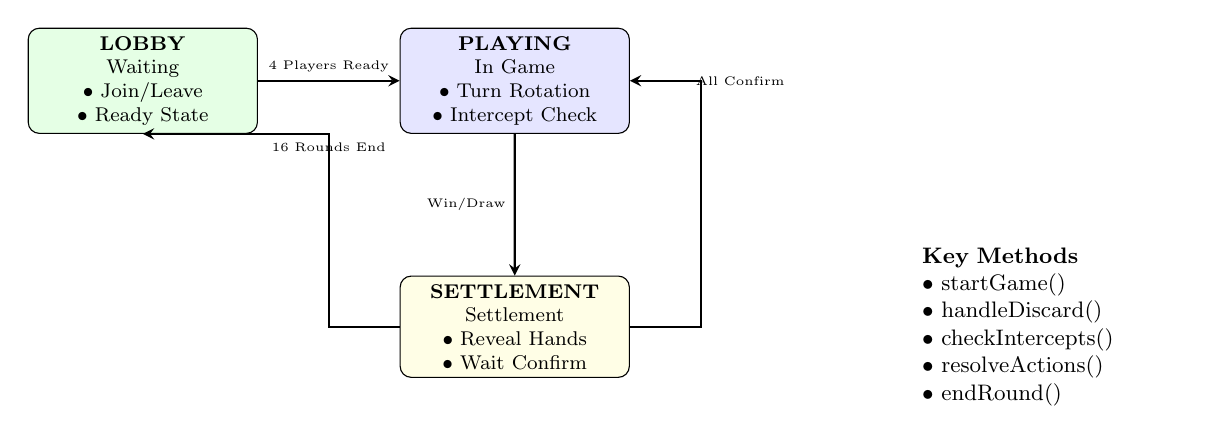
\begin{tikzpicture}[node distance=2cm, scale=0.9, every node/.style={transform shape}]
  \node[rectangle,draw,rounded corners,fill=green!10,text width=3cm,align=center,minimum height=1.3cm,font=\footnotesize] (l) {\textbf{LOBBY}\\Waiting\\$\bullet$ Join/Leave\\$\bullet$ Ready State};
  \node[rectangle,draw,rounded corners,fill=blue!10,text width=3cm,align=center,minimum height=1.3cm,font=\footnotesize,right=of l] (p) {\textbf{PLAYING}\\In Game\\$\bullet$ Turn Rotation\\$\bullet$ Intercept Check};
  \node[rectangle,draw,rounded corners,fill=yellow!10,text width=3cm,align=center,minimum height=1.3cm,font=\footnotesize,below=of p] (s) {\textbf{SETTLEMENT}\\Settlement\\$\bullet$ Reveal Hands\\$\bullet$ Wait Confirm};
  \draw[arr] (l) -- (p) node[midway,above,font=\tiny] {4 Players Ready};
  \draw[arr] (p) -- (s) node[midway,left,font=\tiny] {Win/Draw};
  \draw[arr] (s.east) -- ++(1,0) |- (p.east) node[pos=0.6,right,font=\tiny] {All Confirm};
  \draw[arr] (s.west) -- ++(-1,0) |- (l.south) node[pos=0.5,below,font=\tiny] {16 Rounds End};
  \node[font=\small,right=of s,xshift=2cm,text width=3.5cm] (n) {\textbf{Key Methods}\\$\bullet$ startGame()\\$\bullet$ handleDiscard()\\$\bullet$ checkIntercepts()\\$\bullet$ resolveActions()\\$\bullet$ endRound()};
\end{tikzpicture}
\caption{GameRoom State Machine}
\label{fig:fsm}
\end{figure}

\subsection{Fault Tolerance Mechanisms}

\textbf{Disconnection Reconnection:} Upon client WebSocket disconnection, exponential backoff reconnection initiates with parameters $\tau_0 = 1$\,s, $b = 2$, $N_{\max} = 8$, $\tau_{\max} = 120$\,s. The room ID is persisted via URL query parameter \texttt{?auto\_join=ROOMID\&name=PLAYER}, enabling automatic re-joining upon successful reconnection.

\textbf{Deadlock Prevention:} The server starts a 15-second timeout after distributing action prompts. On timeout, if some players have responded, the system resolves based on existing responses; only when absolutely no one responds does it clear pending state and advance the turn, ensuring the game never permanently stalls due to any player's network failure.

\textbf{Heartbeat and Signal:} The client sends a ping every 10 seconds; the server replies with pong. Round-trip time $\Delta = t_{\text{recv}} - t_{\text{sent}}$ maps to a 4-bar signal indicator: $\Delta < 100$\,ms full bars, $\Delta < 200$\,ms three bars, $\Delta < 400$\,ms two bars, $\Delta \geq 400$\,ms one bar, offline zero bars.

\subsection{Network Latency Measurements}

\begin{table}[H]
\centering
\caption{Network Latency Measurements (ms)}
\label{tab:lat}
\footnotesize
\begin{tabular}{@{}lrrrr@{}}
\toprule
\textbf{Scenario} & \textbf{Min} & \textbf{Avg} & \textbf{P95} & \textbf{Max} \\
\midrule
Local loopback (ws://) & 1 & 3 & 5 & 8 \\
LAN (ngrok, wss://) & 12 & 25 & 45 & 68 \\
4G Mobile & 35 & 72 & 180 & 450 \\
Cross-Province WiFi & 45 & 95 & 210 & 520 \\
\midrule
Agora SD-RTN Voice & 20 & 50 & 120 & 300 \\
\bottomrule
\end{tabular}
\end{table}

\newpage
% ===================================================================
\section{Cross-Platform Compatibility}
% ===================================================================

\subsection{Issue Matrix}

Table~\ref{tab:compat} systematically documents key compatibility issues encountered and resolved during development.

\begin{table}[H]
\centering
\caption{Device Compatibility Issues and Solutions}
\label{tab:compat}
\footnotesize
\begin{tabular}{@{}p{2.5cm}p{1.6cm}p{1.4cm}p{3.5cm}@{}}
\toprule
\textbf{Issue} & \textbf{Platform} & \textbf{Severity} & \textbf{Solution} \\
\midrule
Mobile NAT traversal failure & 4G/5G Mobile & Critical & Agora SD-RTN cloud relay \\
\texttt{<div>} @click silent on iOS & iOS Safari & High & Replace all with \texttt{<button>} + CSS reset \\
AudioContext suspended & iOS Safari & High & Explicit \texttt{ctx.resume()} on user gesture \\
\texttt{100vh} address bar resize & Android Chrome & Medium & \texttt{100dvh} with \texttt{100vh} fallback \\
CSS transform breaks fixed & Desktop scaling & High & Move overlays outside \texttt{game-wrapper} \\
Slow tap (>300ms) missed & iOS/Android & Medium & Tap threshold extended to 500ms \\
\texttt{getUserMedia} no feature detect & HTTP pages & Medium & \texttt{navigator?.mediaDevices?.gUM} guard \\
\texttt{alert()} blocks main thread & All mobile & Low & Replace with Vue overlay components \\
Screen orientation lock fails & iOS $<$ 16 & Low & CSS fallback + silent catch \\
\bottomrule
\end{tabular}
\end{table}

\subsection{iOS Safari Adaptation}

iOS Safari presents several unique constraints: (1) \texttt{getUserMedia} is only available in secure contexts (HTTPS), which GitHub Pages satisfies; (2) AudioContext enters \texttt{suspended} state after creation and must be explicitly resumed in a user-gesture callback; (3) \texttt{@click} events on non-interactive elements (\texttt{<div>}, \texttt{<span>}, \texttt{<img>}) do not fire — only \texttt{<button>} and \texttt{<a href>} possess implicit interactive roles; (4) \texttt{position:fixed} may behave unexpectedly when the software keyboard appears.

TJMJ implements all interactive elements as standard \texttt{<button>} with CSS resets to remove default browser appearance (\texttt{-webkit-appearance:none;} \texttt{padding:0;} \texttt{outline:none;}). AudioContext uses a singleton pattern, created and resumed on first user interaction.

\subsection{Android Chrome Adaptation}

Android Chrome's dynamic address bar causes \texttt{100vh} to include the address bar height. TJMJ uses \texttt{100dvh} (dynamic viewport height) as a replacement, with \texttt{100vh} fallback for older browsers.

\newpage
% ===================================================================
\section{Performance Evaluation}
% ===================================================================

\subsection{Algorithm Performance Benchmarks}

\begin{table}[H]
\centering
\caption{Core Algorithm Performance (Intel i7-13700H 2.4GHz, Node.js v20)}
\label{tab:perf}
\small
\begin{tabular}{@{}lrrrr@{}}
\toprule
\textbf{Algorithm} & \textbf{Avg ($\mu$s)} & \textbf{P95 ($\mu$s)} & \textbf{Max (ms)} & \textbf{Calls/Round} \\
\midrule
Winning-Hand Detection & 85 & 210 & 0.8 & $\sim$200 \\
Ting Detection & 620 & 1450 & 2.1 & $\sim$50 \\
NPC Discard Selection & 340 & 780 & 1.2 & $\sim$40 \\
Online Hand Merge & 12 & 35 & 0.05 & $\sim$80 \\
Message Serialization & 8 & 18 & 0.03 & $\sim$300 \\
\bottomrule
\end{tabular}
\end{table}

\subsection{Online Operation Latency}

\begin{table}[H]
\centering
\caption{End-to-End Online Operation Latency (ms)}
\label{tab:oplat}
\small
\begin{tabular}{@{}lrrr@{}}
\toprule
\textbf{Operation} & \textbf{Local} & \textbf{LAN} & \textbf{Remote} \\
\midrule
Create Room & 5 & 45 & 180 \\
Join Room & 8 & 52 & 210 \\
Discard$\to$State Update & 3 & 25 & 95 \\
Action Prompt$\to$Response & 15 & 80 & 350 \\
Round End$\to$New Round & 25 & 150 & 600 \\
Agora Voice Setup & 200 & 500 & 1500 \\
\bottomrule
\end{tabular}
\end{table}

\newpage
% ===================================================================
\section{Discussion and Future Work}
% ===================================================================

\subsection{Current Limitations}

\begin{enumerate}[nosep]
  \item \textbf{Single-file architecture maintenance cost:} \texttt{App.vue} at 2,602 lines is extremely efficient during rapid iteration, but as functionality grows, splitting into multiple independent components will improve long-term maintainability.
  \item \textbf{Heuristic AI lacks strategic depth:} The current NPC strategy is based on fixed weight rules and cannot learn opponent styles or adapt to complex situations. Deep reinforcement learning agents hold promise for significantly enhancing gameplay.
  \item \textbf{Sound effect assets missing:} 34 pre-recorded mp3 files (27 tile names + 7 action words) have not yet been produced; the system currently falls back entirely to browser TTS synthesis, with unsatisfactory voice quality and response latency.
\end{enumerate}

\subsection{Future Research Directions}

\begin{itemize}[nosep]
  \item \textbf{Deep reinforcement learning mahjong agent:} Train using PPO algorithms in self-play environments, combined with Monte Carlo Tree Search (MCTS) to improve decision quality, targeting human-expert-level performance.
  \item \textbf{Distributed game server:} Introduce Redis Pub/Sub for cross-Node.js process broadcast synchronization, with load balancing for horizontal scaling to support thousands of concurrent rooms.
  \item \textbf{Progressive Web App (PWA):} Implement Service Workers for offline caching, push notifications, and home screen installation, delivering a near-native mobile experience.
  \item \textbf{Replay system and intelligent spectating:} Record complete per-round operation logs, supporting timeline replay, multi-perspective auto-switching, and GPT-based game commentary generation.
  \item \textbf{Cross-platform desktop client:} Use Electron or Tauri to wrap the web frontend as a desktop application with system-level shortcuts, notifications, and improved performance.
\end{itemize}

% ===================================================================
\section*{Appendix: Message Sequence Example}
\addcontentsline{toc}{section}{Appendix: Message Sequence Example}

The following illustrates a complete "discard → intercept → execute → discard" message round-trip for online play, involving 5 messages across 3 participants (P0, P1, Server).

\begin{figure}[H]
\centering
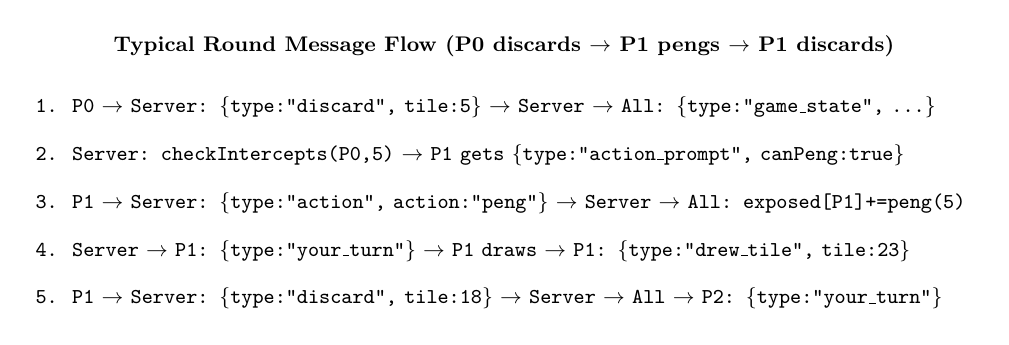
\begin{tikzpicture}[node distance=0.55cm, scale=0.85, every node/.style={transform shape}]
  \node[font=\small\bfseries] (t) {Typical Round Message Flow (P0 discards $\to$ P1 pengs $\to$ P1 discards)};
  \node[font=\small,below=0.35cm of t,text width=14cm] (a) {\texttt{1.\ \ P0 $\to$ Server: \{type:"discard", tile:5\} $\to$ Server $\to$ All: \{type:"game\_state", ...\}}};
  \node[font=\small,below=0.15cm of a,text width=14cm] (b) {\texttt{2.\ \ Server: checkIntercepts(P0,5) $\to$ P1 gets \{type:"action\_prompt", canPeng:true\}}};
  \node[font=\small,below=0.15cm of b,text width=14cm] (c) {\texttt{3.\ \ P1 $\to$ Server: \{type:"action", action:"peng"\} $\to$ Server $\to$ All: exposed[P1]+=peng(5)}};
  \node[font=\small,below=0.15cm of c,text width=14cm] (d) {\texttt{4.\ \ Server $\to$ P1: \{type:"your\_turn"\} $\to$ P1 draws $\to$ P1: \{type:"drew\_tile", tile:23\}}};
  \node[font=\small,below=0.15cm of d,text width=14cm] (e) {\texttt{5.\ \ P1 $\to$ Server: \{type:"discard", tile:18\} $\to$ Server $\to$ All $\to$ P2: \{type:"your\_turn"\}}};
\end{tikzpicture}
\caption{Online Round Message Sequence}
\label{fig:msgseq}
\end{figure}

\newpage
% ===================================================================
\section{Project Engineering Structure}
% ===================================================================

\subsection{Complete Project Directory Structure}

Figure~\ref{fig:tree} presents the complete file organization of the TJMJ project in tree form.

\begin{figure}[H]
\centering
\small
\begin{verbatim}
TJMJ/                                       # Project Root
├── .git/                                   # Git Version Control
├── .github/workflows/deploy.yml            # GitHub Actions CI
├── start-all.bat                           # One-Click Launch Script
├── stop-all.bat                            # Stop Script
├── readme.md                               # Project Introduction & Rules
├── ARCHITECTURE.md                         # Full-Stack Architecture Doc
│
├── docs/manual/                            # ★ Manual Workspace
│   ├── pictures/                           #    Game Screenshots
│   ├── TJMJ_Technical_Manual_EN.tex        #    English LaTeX Source
│   ├── TJMJ_Technical_Manual_EN.pdf        #    English PDF
│   ├── TJMJ_Technical_Manual_CN.tex        #    Chinese LaTeX Source
│   └── TJMJ_Technical_Manual_CN.pdf        #    Chinese PDF
│
├── frontend/                               # ★ Vue 3 Frontend (SPA)
│   ├── index.html                          #    HTML Entry
│   ├── vite.config.js                      #    Vite Config (base: /TJMJ/)
│   ├── src/
│   │   ├── App.vue                         #    ★ Main Component (2602 lines)
│   │   ├── main.js                         #    Vue Entry Point
│   │   ├── core/                           #    Game Engine
│   │   ├── ai/                             #    Artificial Intelligence
│   │   ├── network/                        #    Network Layer
│   │   └── utils/                          #    Utilities
│   └── public/
│       ├── images/                         #    Tile Assets
│       ├── docs/                           #    In-Game PDF + Video
│       └── *.mp3                           #    BGM Music
│
├── server/                                 # ★ Node.js Game Server
│   ├── index.js                            #    WebSocket Entry (247 lines)
│   ├── GameRoom.js                         #    Room State Machine (494 lines)
│   └── game/                               #    Game Logic (server-authoritative)
│
└── other/                                  # Local Tools (ngrok + backups)
\end{verbatim}
\caption{Complete Project File Tree}
\label{fig:tree}
\end{figure}

\newpage
% ===================================================================
\section*{Appendix A: Scoring Addendum}
\addcontentsline{toc}{section}{Appendix A: Scoring Addendum}

\begin{table}[H]
\centering
\caption{Complete Hand Scoring (Self-Draw + Zha Niao)}
\label{tab:score_full}
\footnotesize
\begin{tabular}{@{}llcccc@{}}
\toprule
\textbf{Hand Type} & \textbf{Fan} & \textbf{Hit One} & \textbf{All Hit} & \textbf{Miss Pay} & \textbf{Hit Pay} \\
\midrule
Hei Tian Hu  & 2 & 8  & 12 & 2  & 4  \\
Di Hu        & 2 & 8  & 12 & 2  & 4  \\
Tian Hu      & 3 & 12 & 18 & 3  & 6  \\
Tian Tian Hu & 5 & 20 & 30 & 5  & 10 \\
Peng Peng Hu & 2 & 8  & 12 & 2  & 4  \\
Qing Yi Se   & 2 & 8  & 12 & 2  & 4  \\
Qi Xiao Dui  & 2 & 8  & 12 & 2  & 4  \\
JiangJiang Hu& 2 & 8  & 12 & 2  & 4  \\
Qi Shou Hu   & 2 & 8  & 12 & 2  & 4  \\
Kai Gang     & 2 & 8  & 12 & 2  & 4  \\
Ying Zhuang  & 2$\times$ & 8  & 12 & 2  & 4  \\
Di Hu Dai Tuo& 3 & 12 & 18 & 3  & 6  \\
Qi Shou Ting & 2 & 8  & 12 & 2  & 4  \\
\bottomrule
\end{tabular}
\end{table}

\newpage
% ===================================================================
\section*{Appendix B: Environment Setup}
\addcontentsline{toc}{section}{Appendix B: Environment Setup}

\begin{verbatim}
# 1. Install dependencies
cd frontend && npm install
cd ../server && npm install

# 2. Set Agora credentials (for voice)
set AGORA_APP_CERT=your_certificate_here

# 3. One-click launch (Windows)
.\start-all.bat
# → Window 1: Server @ :8080
# → Window 2: Frontend @ :5173
# → Window 3: ngrok tunnel

# 4. Deploy frontend
cd frontend && npm run build && npm run deploy

# 5. Compile manual
cd docs/manual
xelatex TJMJ_Technical_Manual_EN.tex  # ×3
\end{verbatim}

\newpage
% ===================================================================
\section*{Appendix C: Game Interface Showcase}
\addcontentsline{toc}{section}{Appendix C: Game Interface Showcase}

\begin{figure}[H]
\centering
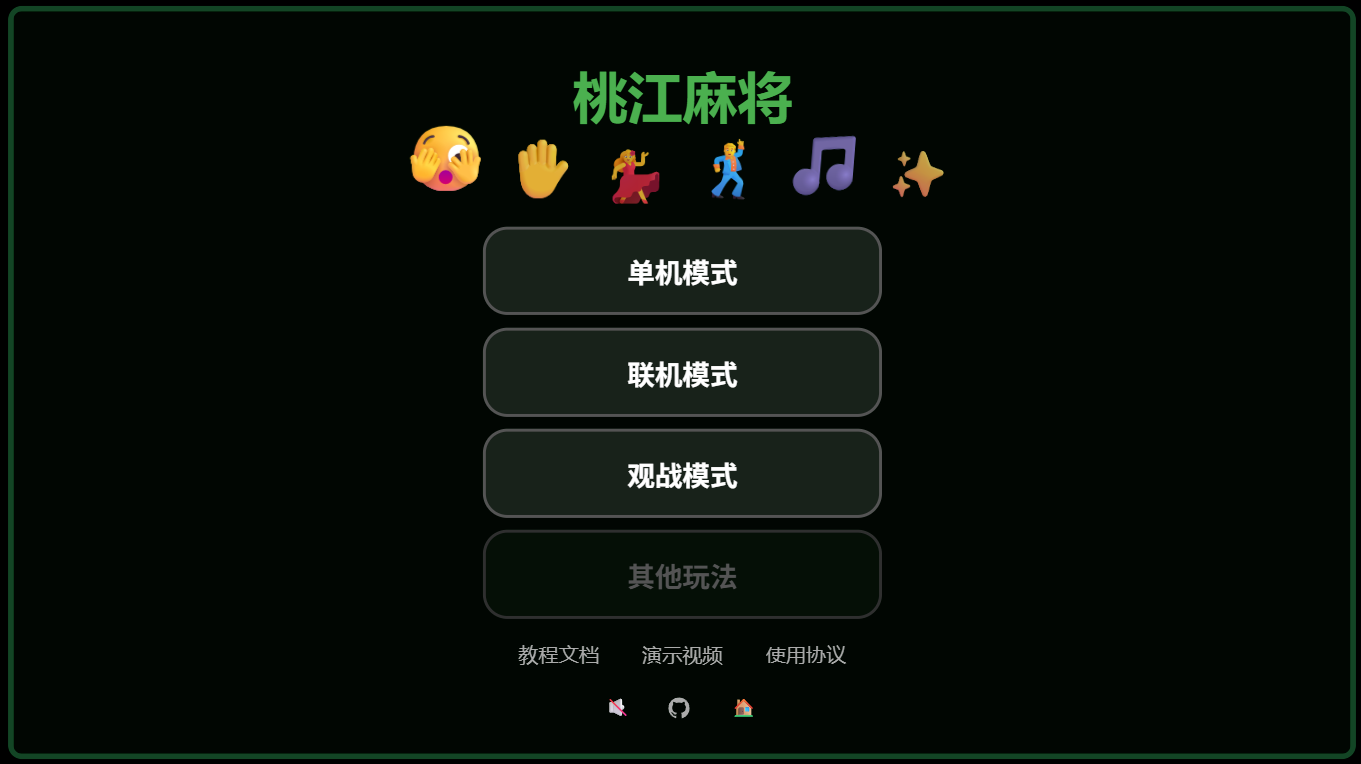
\includegraphics[width=0.92\textwidth]{pictures/1.主界面.png}
\caption{Main Menu — Mode selection with single-player, multiplayer, and spectator options.}
\end{figure}

\begin{figure}[H]
\centering
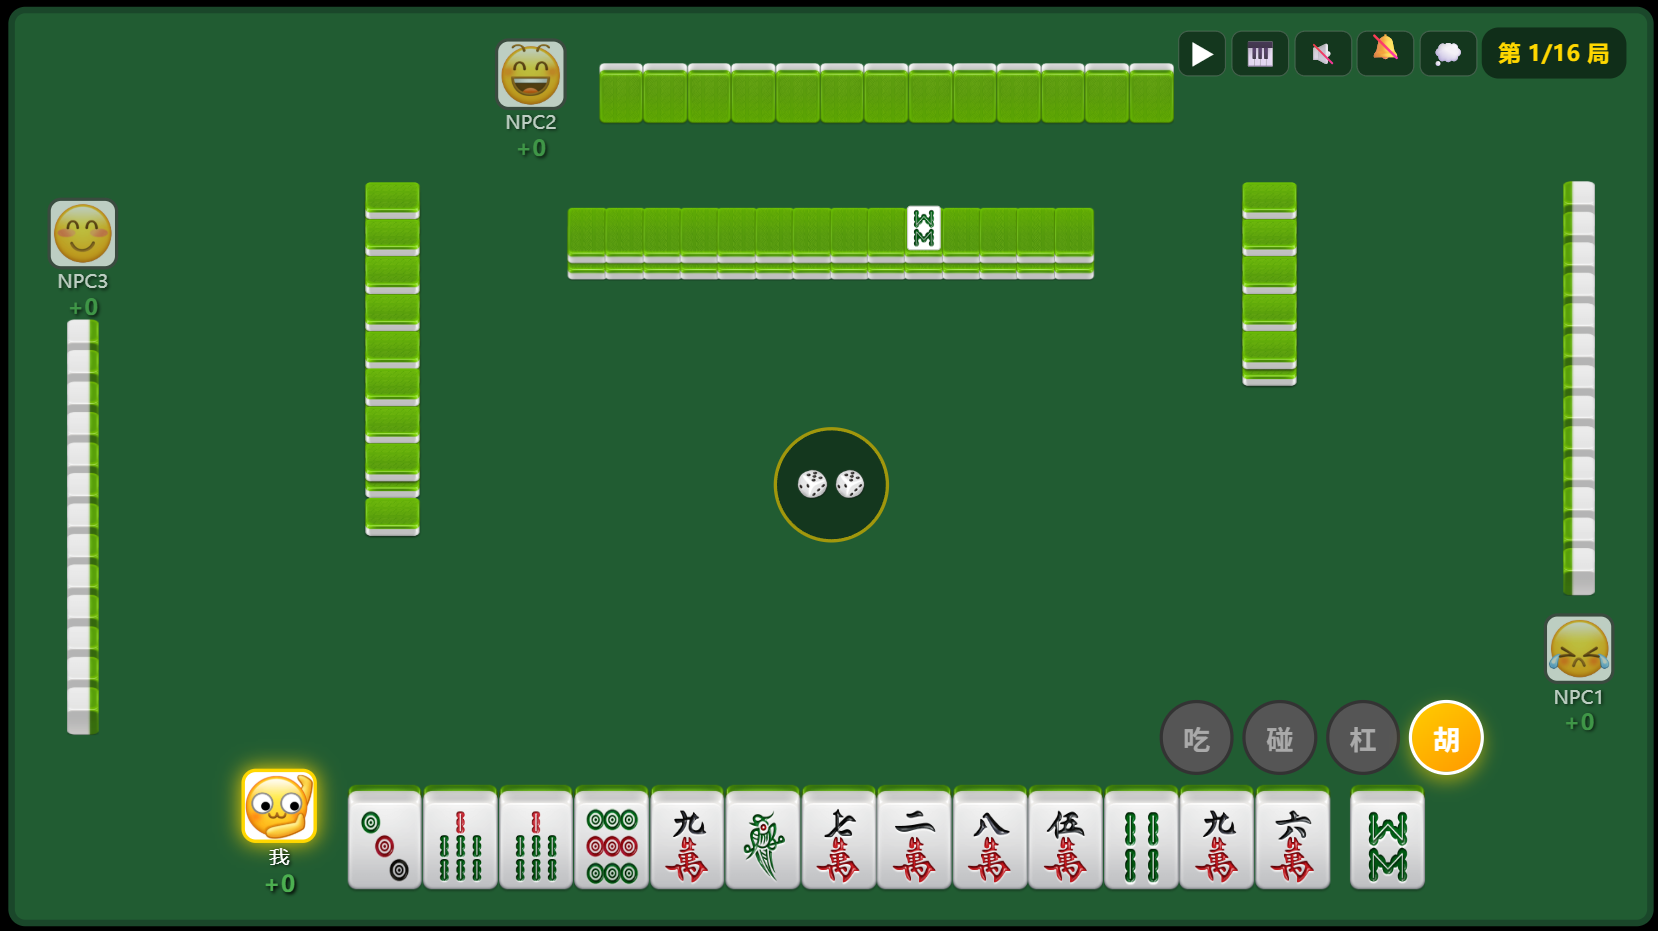
\includegraphics[width=0.92\textwidth]{pictures/2.单机模式.png}
\caption{Single-Player Mode — Player (bottom) versus three AI opponents, showing all four hands, discard pool, dice, and action buttons.}
\end{figure}

\begin{figure}[H]
\centering
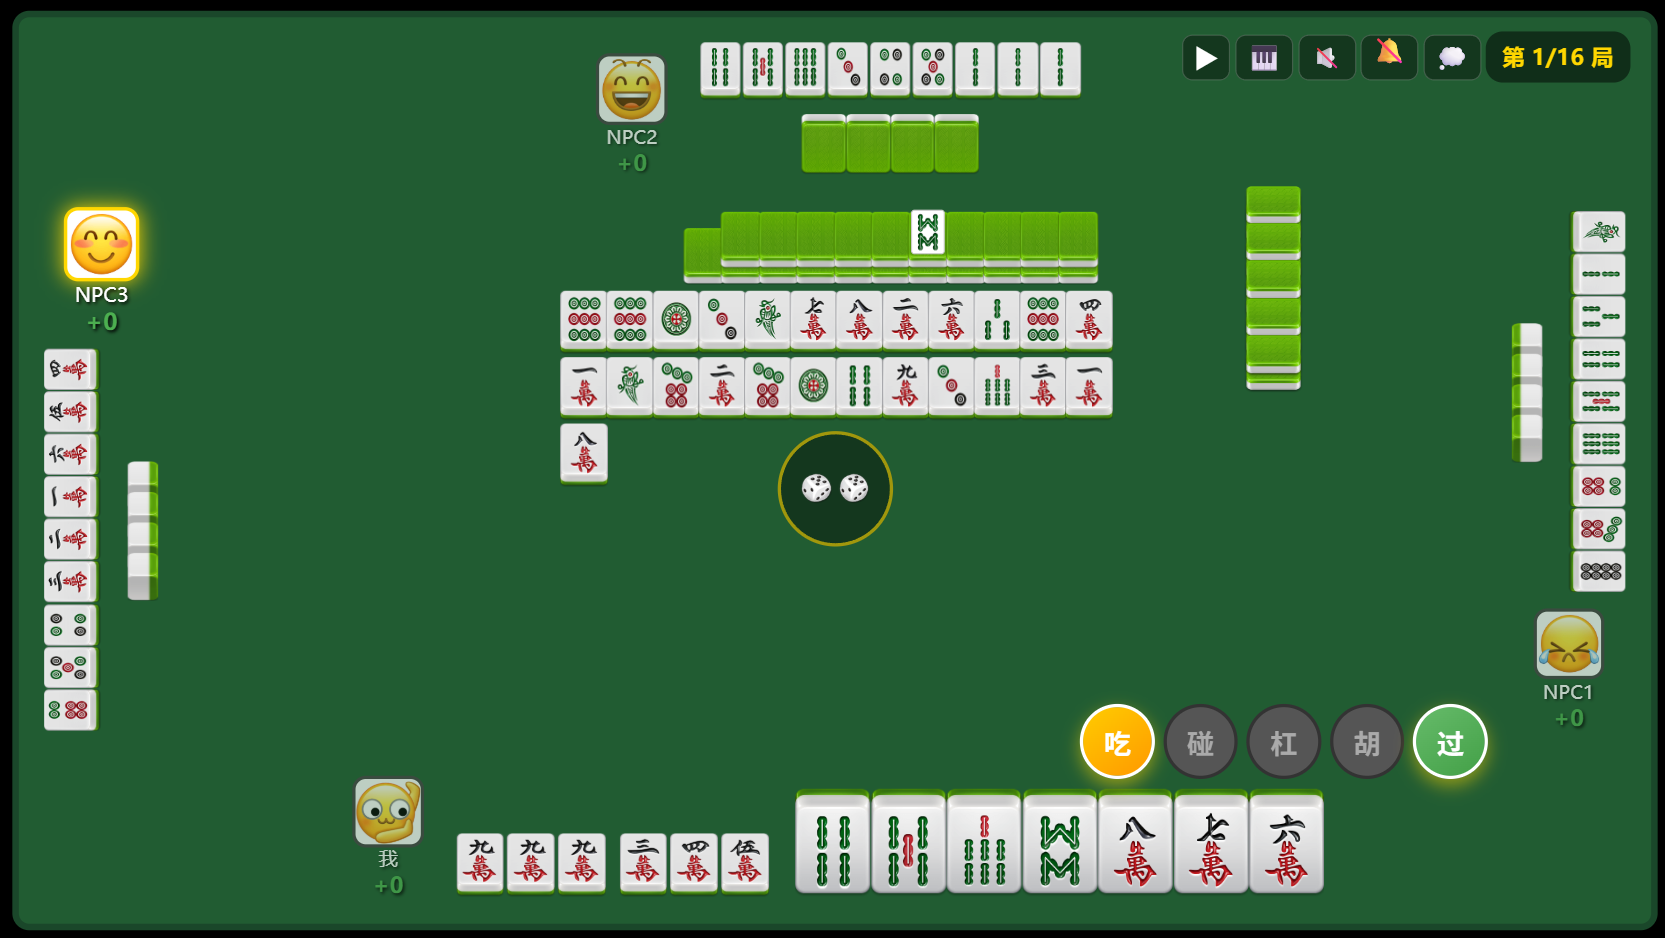
\includegraphics[width=0.92\textwidth]{pictures/2.单机模式对局过程.png}
\caption{Round Settlement — All four hands revealed with cumulative scores; winner highlighted.}
\end{figure}

\begin{figure}[H]
\centering
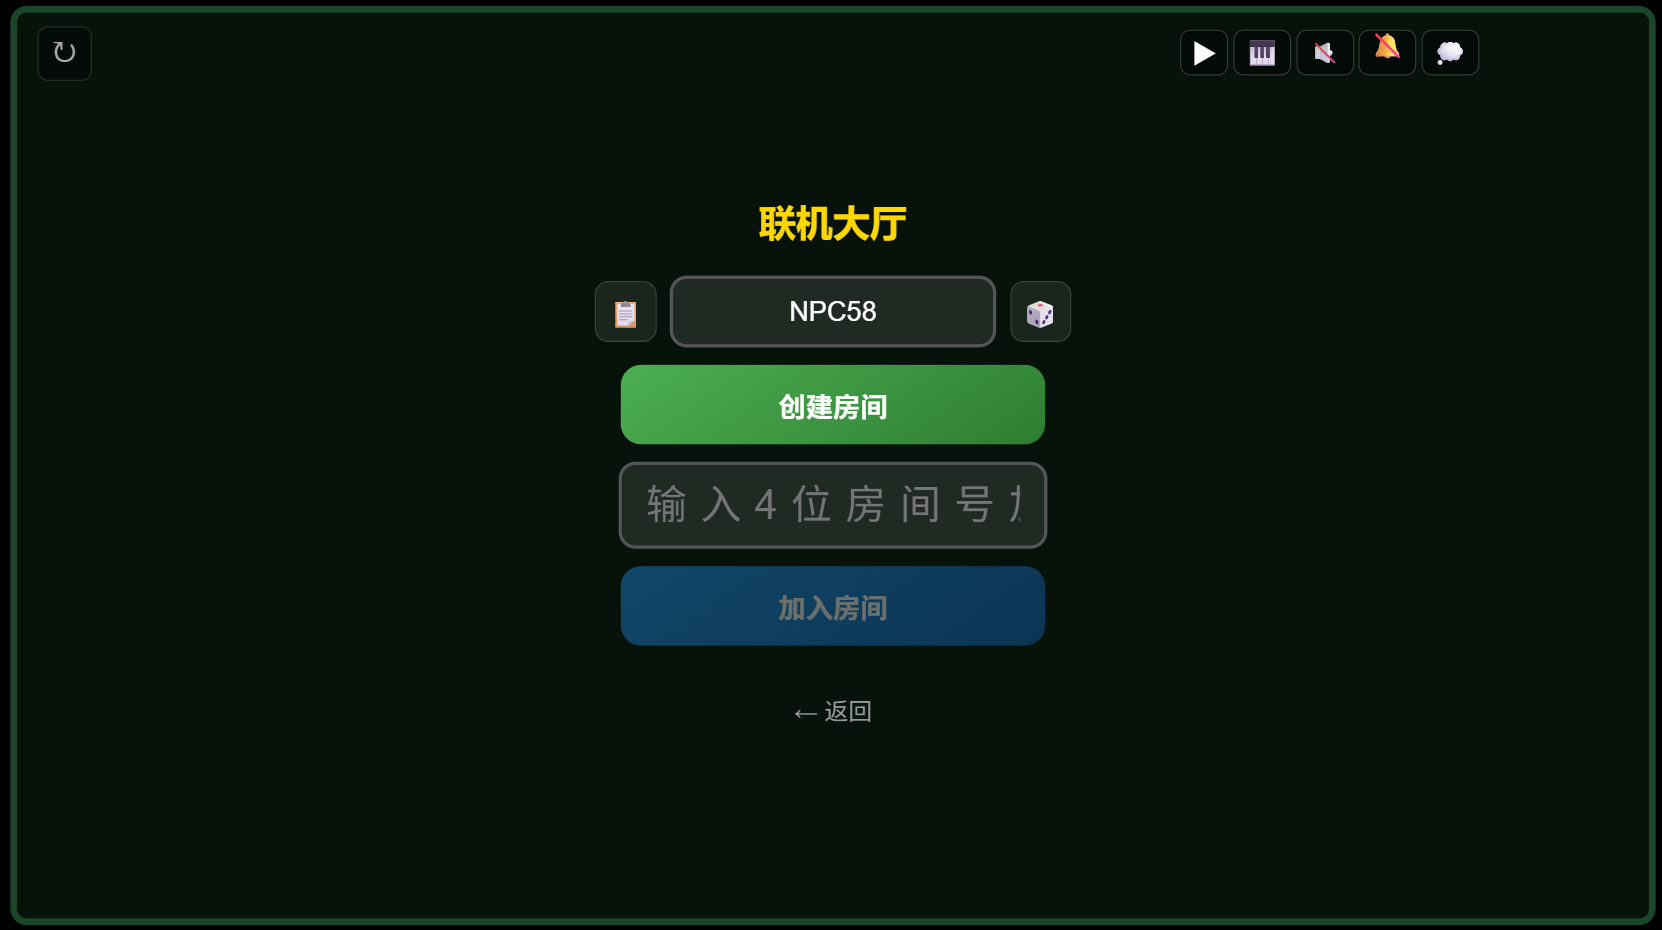
\includegraphics[width=0.92\textwidth]{pictures/3.联机大厅.png}
\caption{Online Lobby — Nickname input with memory chips and random nickname, create or join room by 4-digit code.}
\end{figure}

\begin{figure}[H]
\centering
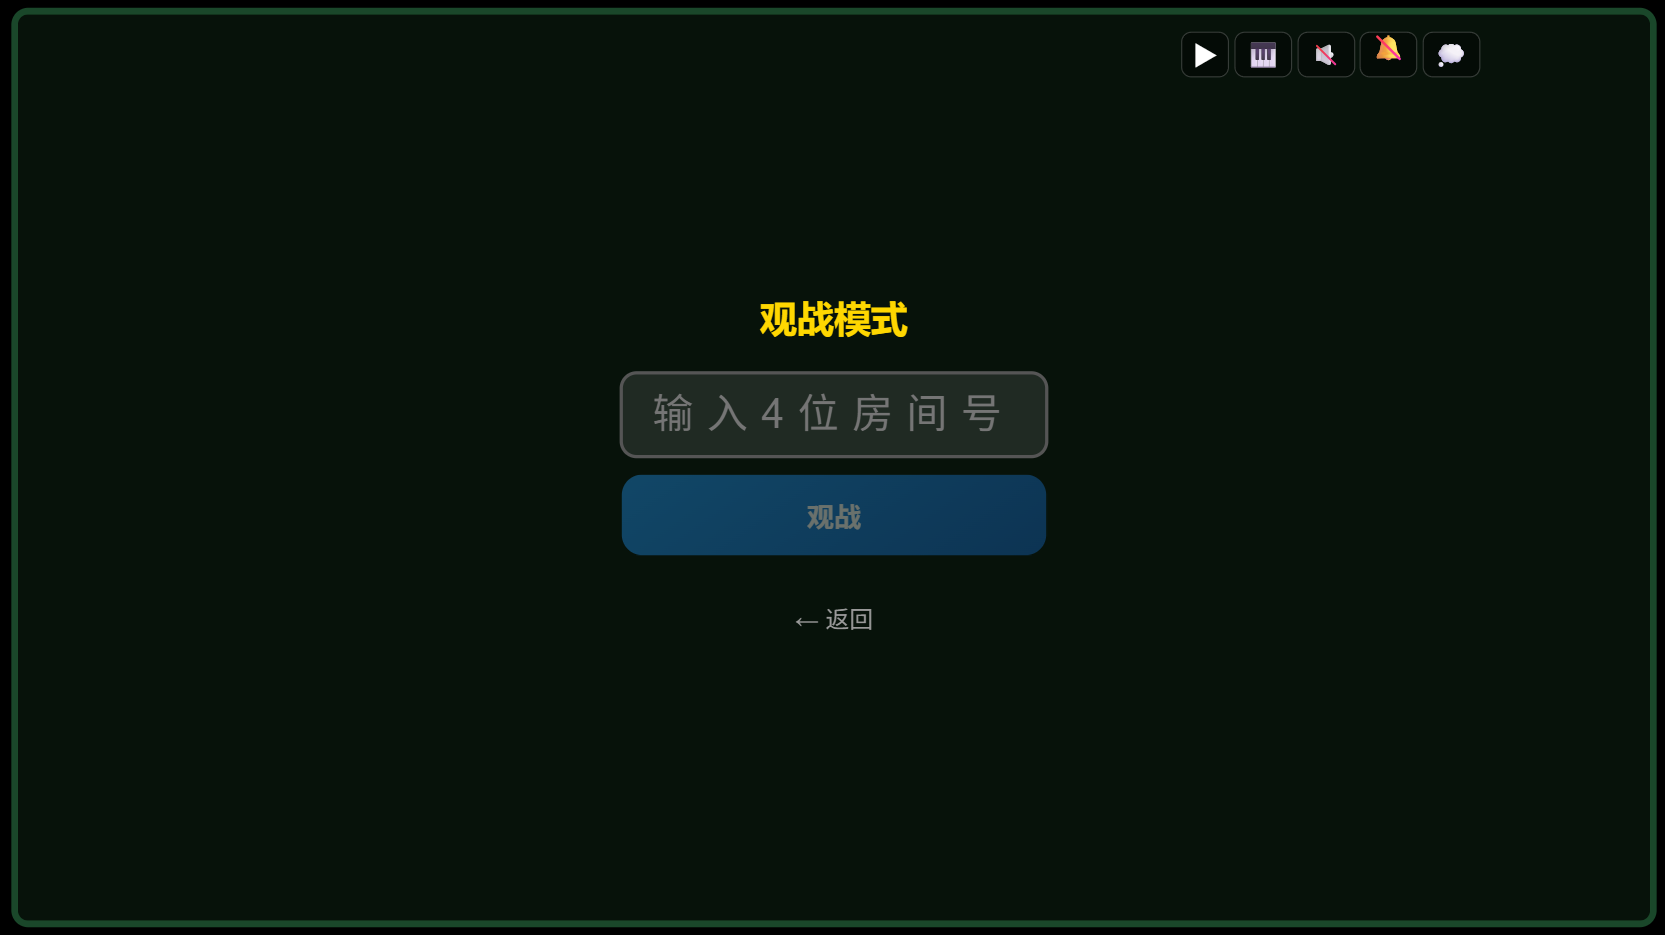
\includegraphics[width=0.92\textwidth]{pictures/5.观战模式.png}
\caption{Spectator Mode — Watch ongoing games by entering a 4-digit room code; click any player avatar to switch viewing perspective.}
\end{figure}

\begin{figure}[H]
\centering
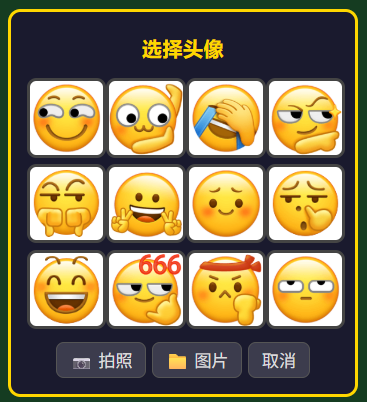
\includegraphics[width=0.92\textwidth]{pictures/功能介绍：头像选择.png}
\caption{Avatar Selection — 12 preset emoji avatars plus camera/local image upload; saved to localStorage.}
\end{figure}

\begin{figure}[H]
\centering
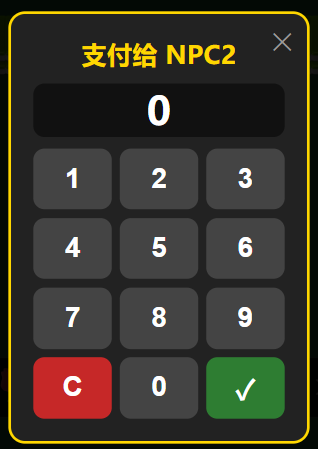
\includegraphics[width=0.92\textwidth]{pictures/功能介绍：手动支付给分.png}
\caption{Manual Score Transfer — Tap any player's score area to open a numpad for flexible settlement.}
\end{figure}

\begin{figure}[H]
\centering

\includegraphics[width=0.92\textwidth]{pictures/功能介绍：游戏界面右上角按钮和对局情况.png}
\caption{Top-Right Controls — Song skip, BGM toggle, microphone (Agora voice with level indicator), and chat danmaku button.}
\end{figure}

\begin{figure}[H]
\centering

\includegraphics[width=0.92\textwidth]{pictures/功能介绍：点击玩家头像交互.png}
\caption{Player Avatar Interaction — Send emojis (rose/poop/egg/bomb/money) to other players with flying animation; money emoji transfers 1 point.}
\end{figure}

\newpage
% ===================================================================
\section*{References}
\addcontentsline{toc}{section}{References}

\begin{enumerate}[nosep]
  \item RFC 6455: The WebSocket Protocol. IETF, 2011.
  \item WebRTC 1.0: Real-Time Communication Between Browsers. W3C, 2021.
  \item Vue.js 3.5 Documentation. \url{https://vuejs.org/}, 2025.
  \item Vite 8.0 Documentation. \url{https://vitejs.dev/}, 2025.
  \item Node.js v20 Documentation. OpenJS Foundation, 2025.
  \item Agora Real-Time Voice SDK. \url{https://www.agora.io/}, 2025.
  \item OpenMajiang Project. \url{https://gitee.com/mirrors/OpenMajiang}.
  \item V. Mnih et al. ``Human-level control through deep reinforcement learning.'' Nature, 518(7540):529--533, 2015.
  \item D. Silver et al. ``Mastering the game of Go with deep neural networks and tree search.'' Nature, 529(7587):484--489, 2016.
\end{enumerate}

\vfill
\begin{center}
\rule{\linewidth}{0.4pt}
{\small\textit{TJMJ Technical Manual v3.0 English Edition — \today}}\\[2pt]
{\tiny Taojiang Classic Wang Mahjong $\,\mid\,$ Full-Stack Real-Time Web $\,\mid\,$ Fully Open Source}
\end{center}

\end{document}
